\documentclass[10pt,aspectratio=169]{beamer}
\usepackage[T1]{fontenc}
\usepackage{booktabs}
\usepackage{colortbl}
\usepackage{xcolor}
\usepackage{tikz}
\usetikzlibrary{arrows,shapes,positioning,fit,backgrounds}
\usetheme{metropolis}

% Color definitions for consistency
\definecolor{darkblue}{RGB}{23, 73, 137}
\definecolor{accent}{RGB}{0, 163, 224}
\definecolor{lightblue}{RGB}{230, 242, 255}

\title{Challenges of Implementing Electronic Health Records (EHRs) in Rural and Resource-Constrained Settings}
\subtitle{SDS6210 – Informatics for Health \\ MSc Public Health Data Science}
\author{Cavin Otieno}
\institute{Department of Public Health}
\date{\today}

\begin{document}

%=======================================================================
% TITLE FRAME
%=======================================================================
{
\setbeamertemplate{footline}{}
\begin{frame}
    \titlepage
\end{frame}
}

%=======================================================================
% OUTLINE
%=======================================================================
\section{Outline}
\begin{frame}{Presentation Outline}
    \begin{enumerate}
        \item Definitions and Conceptual Framework
        \item Infrastructure and Connectivity Challenges
        \item Human Resources and Digital Skills Gap
        \item Financial and Sustainability Constraints
        \item Data Quality, Security, and Privacy Issues
        \item Governance, Policy, and Regulatory Challenges
        \item Sociocultural and Organizational Factors
        \item Implications for Quality, Equity, and Outcomes
        \item Implementation and Policy Recommendations
        \item Conclusions
    \end{enumerate}
\end{frame}

%=======================================================================
% SECTION 1: DEFINITIONS AND CONCEPTUAL FRAMEWORK
%=======================================================================
\section{Definitions and Conceptual Framework}
\subsection{Definition of Electronic Health Records}

\begin{frame}{What are Electronic Health Records?}
    \begin{block}{WHO Definition}
        An electronic health record (EHR) is a ``systematic collection of electronic health information about individual patients or populations'' that is ``capable of being shared across different health care settings'' through networked, enterprise-wide information systems or other information networks and exchanges \cite{who2009}.
    \end{block}
    
    \pause
    
    \begin{itemize}
        \item \textbf{Scope}: Goes beyond basic patient demographics to include medical history, medications, allergies, immunization status, laboratory results, vital signs, and billing information
        \item \textbf{Interoperability}: The capacity for EHR systems to exchange and make use of information across organizational and geographic boundaries
        \item \textbf{Purpose}: Support continuity of care, clinical decision-making, public health surveillance, health system planning, and research
    \end{itemize}
\end{frame}

\begin{frame}{EHRs in Health Systems Strengthening}
    \begin{center}
        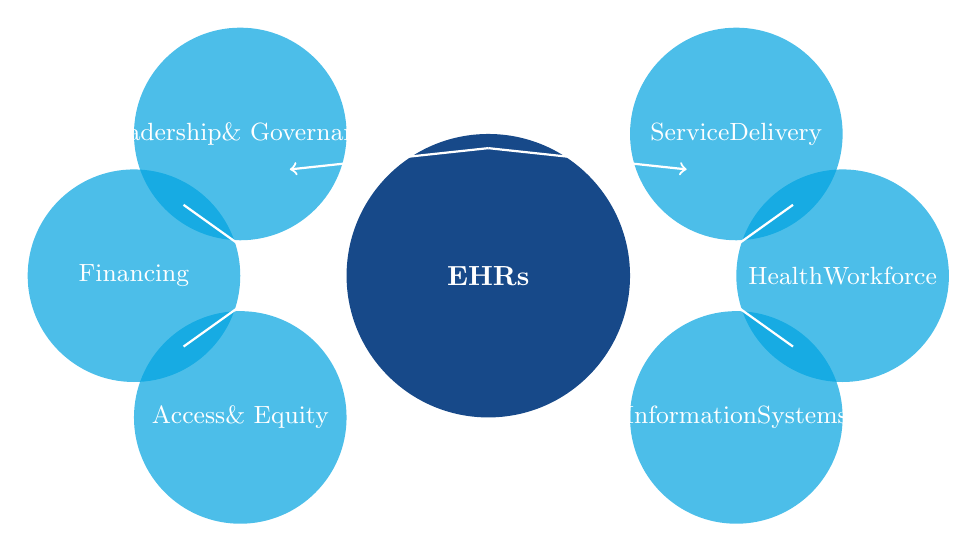
\begin{tikzpicture}[scale=0.9]
            % Central hexagon
            \draw[fill=darkblue, draw=none] (0,0) circle (2cm);
            \node[white, font=\bfseries] at (0,0) {EHRs};
            
            % Outer circles
            \draw[fill=accent, draw=none, opacity=0.7] (3.5,2) circle (1.5cm);
            \node[white, font=\small] at (3.5,2) {Service\\Delivery};
            
            \draw[fill=accent, draw=none, opacity=0.7] (5,0) circle (1.5cm);
            \node[white, font=\small] at (5,0) {Health\\Workforce};
            
            \draw[fill=accent, draw=none, opacity=0.7] (3.5,-2) circle (1.5cm);
            \node[white, font=\small] at (3.5,-2) {Information\\Systems};
            
            \draw[fill=accent, draw=none, opacity=0.7] (-3.5,-2) circle (1.5cm);
            \node[white, font=\small] at (-3.5,-2) {Access\\\& Equity};
            
            \draw[fill=accent, draw=none, opacity=0.7] (-5,0) circle (1.5cm);
            \node[white, font=\small] at (-5,0) {Financing};
            
            \draw[fill=accent, draw=none, opacity=0.7] (-3.5,2) circle (1.5cm);
            \node[white, font=\small] at (-3.5,2) {Leadership\\\& Governance};
            
            % Arrows connecting
            \draw[->, thick, white] (0,1.8) -- (2.8,1.5);
            \draw[->, thick, white] (0,1.8) -- (-2.8,1.5);
            \draw[->, thick, white] (4.3,1) -- (2.2,-0.5);
            \draw[->, thick, white] (4.3,-1) -- (2.2,0.5);
            \draw[->, thick, white] (-4.3,-1) -- (-2.2,0.5);
            \draw[->, thick, white] (-4.3,1) -- (-2.2,-0.5);
        \end{tikzpicture}
    \end{center}
    
    \smallskip
    
    EHRs intersect with all six WHO health systems building blocks, making their implementation particularly complex in resource-constrained environments \cite{who2007}.
\end{frame}

\begin{frame}{Systems Thinking Framework for EHR Implementation}
    \begin{itemize}
        \item \textbf{Linear vs. Systems Approach}: Traditional implementation often assumes a linear ``deploy and adopt'' model; systems thinking recognizes recursive feedback loops, emergent properties, and interdependencies
        \item \textbf{Complexity Science Perspective}: EHR implementation in LMICs represents a complex adaptive system with multiple interacting agents (patients, providers, administrators, policymakers, technology vendors)
        \item \textbf{Conceptual Model}: The CHIMERA framework (Context, Hardware, Infrastructure, Management, End-users, Regulations, Adaptation) provides a lens for analyzing EHR implementation challenges in low-resource settings \cite{luna2014}
        \item \textbf{Feedback Loops}: Infrastructure investments affect workforce capacity; workforce training affects adoption rates; adoption affects data quality; data quality affects perceived value and continued investment
    \end{itemize}
\end{frame}

%=======================================================================
% SECTION 2: INFRASTRUCTURE AND CONNECTIVITY
%=======================================================================
\section{Infrastructure and Connectivity Challenges}

\begin{frame}{Power Supply and Reliability}
    \begin{columns}
        \begin{column}{0.5\textwidth}
            \begin{block}{The Problem}
                Rural health facilities in LMICs frequently experience:
                \begin{itemize}
                    \item Unreliable grid electricity (average 8-12 hours/day in sub-Saharan Africa)
                    \item Voltage fluctuations damaging sensitive equipment
                    \item Complete absence of electricity in remote areas
                    \item Limited or no backup power systems
                \end{itemize}
            \end{block}
        \end{column}
        \begin{column}{0.5\textwidth}
            \begin{block}{Case Study: Rural India}
                A study across 96 primary health centers in Rajasthan found that 67\% reported daily power outages exceeding 4 hours, making consistent EHR operation nearly impossible without substantial solar or generator backup \cite{agarwal2019}.
            \end{block}
        \end{column}
    \end{columns}
    
    \pause
    
    \begin{block}{Implications}
        Unreliable power creates ``digital deserts'' where paper-based records remain the only viable option, perpetuating the very data fragmentation that EHRs are meant to solve.
    \end{block}
\end{frame}

\begin{frame}{Connectivity and Internet Infrastructure}
    \begin{center}
        \begin{tabular}{@{}lp{6cm}@{}}
            \toprule
            \textbf{Challenge} & \textbf{Impact on EHR Implementation} \\
            \midrule
            Limited broadband access & Prevents cloud-based EHR systems; slows synchronization of local databases \\
            High latency connections & Makes real-time data entry and verification impractical \\
            Intermittent connectivity & Forces hybrid paper-digital workflows that increase error rates \\
            Cost of data transmission & Makes large file uploads (e.g., diagnostic images) prohibitive \\
            \bottomrule
        \end{tabular}
    \end{center}
    
    \pause
    
    \begin{block}{African Context}
        According to ITU data, while mobile network coverage reaches approximately 85\% of the African population, broadband connectivity in rural areas remains below 30\% \cite{itu2022}. This ``last mile'' problem means even where networks exist, the bandwidth required for EHR operations is unavailable at the point of care.
    \end{block}
\end{frame}

\begin{frame}{Hardware and Device Constraints}
    \begin{columns}
        \begin{column}{0.45\textwidth}
            \begin{itemize}
                \item \textbf{Cost barriers}: High capital costs for computers, servers, and peripheral devices
                \item \textbf{Procurement challenges}: Long procurement cycles; difficulty sourcing replacements
                \item \textbf{Maintenance gaps}: Lack of local technical support; prolonged downtime
                \item \textbf.Device obsolescence}: Old operating systems incompatible with modern EHR software
                \item \textbf{Environmental factors}: Heat, humidity, and dust accelerate hardware degradation
            \end{itemize}
        \end{column}
        \begin{column}{0.55\textwidth}
            \begin{block}{Mozambique Case Study}
                TheSistema Nacional de Saúde (SNS) EHR implementation found that hardware maintenance costs consumed 40\% of the total IT budget, with an average equipment lifespan 50\% shorter than manufacturer specifications due to tropical climate conditions \cite{o'donovan2019}.
            \end{block}
        \end{column}
    \end{columns}
    
    \pause
    
    \begin{block}{Mobile Health (mHealth) Alternative}
        Mobile-based EHR solutions (using smartphones and tablets) offer lower cost and greater flexibility but introduce their own challenges including small screen interfaces, battery life limitations, and device fragmentation.
    \end{block}
\end{frame}

%=======================================================================
% SECTION 3: HUMAN RESOURCES AND DIGITAL SKILLS
%=======================================================================
\section{Human Resources and Digital Skills}

\begin{frame}{The Health Workforce Crisis in LMICs}
    \begin{center}
        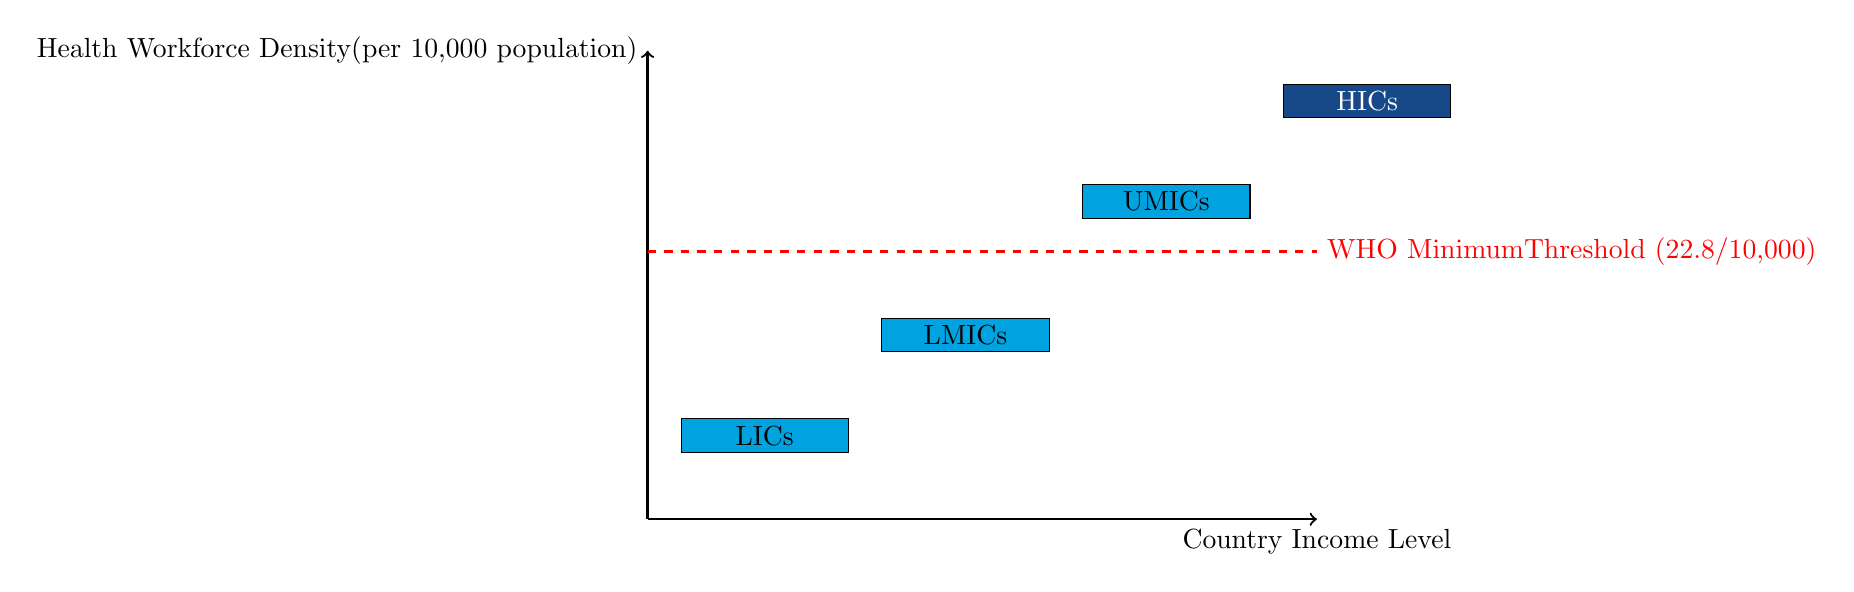
\begin{tikzpicture}[scale=0.85]
            \draw[->, thick] (0,0) -- (10,0) node[below] {Country Income Level};
            \draw[->, thick] (0,0) -- (0,7) node[left] {Health Workforce Density\\ (per 10,000 population)};
            
            % Bars
            \draw[fill=accent] (0.5,1) rectangle (3,1.5) node[pos=.5, black] {LICs};
            \draw[fill=accent] (3.5,2.5) rectangle (6,3) node[pos=.5, black] {LMICs};
            \draw[fill=accent] (6.5,4.5) rectangle (9,5) node[pos=.5, black] {UMICs};
            \draw[fill=darkblue] (9.5,6) rectangle (12,6.5) node[pos=.5, white] {HICs};
            
            % WHO threshold
            \draw[dashed, red, thick] (0,4) -- (10,4) node[right, red] {WHO Minimum\\Threshold (22.8/10,000)};
        \end{tikzpicture}
    \end{center}
    
    \smallskip
    
    According to WHO, 57 countries (36 in sub-Saharan Africa) have critical health workforce shortages below the minimum threshold of 22.8 health workers per 10,000 population \cite{who2020}. This workforce crisis directly constrains EHR adoption.
\end{frame}

\begin{frame}{Digital Literacy and Computer Skills Gap}
    \begin{columns}
        \begin{column}{0.5\textwidth}
            \begin{block}{Training Challenges}
                \begin{itemize}
                    \item Variable computer literacy among health workers, particularly older staff
                    \item Limited exposure to structured data entry and management principles
                    \item Insufficient training time due to clinical workload pressures
                    \item Training often conducted in urban centers, excluding rural workers
                    \item Rapid staff turnover requiring repeated training cycles
                \end{itemize}
            \end{block}
        \end{column}
        \begin{column}{0.5\textwidth}
            \begin{block}{Kenya Case Study}
                An evaluation of the KenyaEMR system in Nyanza Province found that 45\% of health workers reported ``difficulty using computers'' as a major barrier to adoption, with training duration averaging only 2 days per facility \cite{ Were2013}.
            \end{block}
        \end{column}
    \end{columns}
    
    \pause
    
    \begin{block}{Critical Insight}
        Technology adoption models developed in high-income countries often overestimate baseline digital literacy. In many LMIC rural settings, EHR implementation requires foundational computer skills training before introducing the system itself.
    \end{block}
\end{frame}

\begin{frame}{Specialized Informatics Capacity}
    \begin{itemize}
        \item \textbf{Health Informatics Experts}: There is a severe global shortage of professionals with combined expertise in health sciences, information systems, and public health—particularly acute in LMICs
        \item \textbf{Local IT Support}: Rural facilities often lack on-site IT personnel, leading to delayed troubleshooting and extended system downtime
        \item \textbf{Data Management Capacity}: Skills in data analysis, interpretation, and visualization needed to realize EHR benefits are frequently absent at facility level
        \item \textbf{Change Management}: Organizational change management skills essential for successful technology transitions are rarely available
    \end{itemize}
    
    \pause
    
    \begin{block}{Brain Drain Phenomenon}
        Health workers who develop informatics skills often migrate to urban areas or international positions, creating a persistent ``skills drain'' that undermines sustainable capacity building in rural facilities \cite{eksteen2021}.
    \end{block}
\end{frame}

%=======================================================================
% SECTION 4: FINANCIAL AND SUSTAINABILITY CONSTRAINTS
%=======================================================================
\section{Financial and Sustainability Constraints}

\begin{frame}{Cost Structure of EHR Implementation}
    \begin{center}
        \begin{tabular}{@{}lp{6cm}c@{}}
            \toprule
            \textbf{Category} & \textbf{Components} & \textbf{Cost Share} \\
            \midrule
            Capital Costs & Hardware, software licenses, infrastructure & 30-40\% \\
            Implementation & Customization, integration, testing, training & 25-35\% \\
            Operational & Maintenance, updates, support, connectivity & 25-30\% \\
            Indirect & Productivity losses during transition, workflow redesign & 10-15\% \\
            \bottomrule
        \end{tabular}
    \end{center}
    
    \pause
    
    \begin{block}{The Sustainability Challenge}
        Initial implementation grants often cover capital and implementation costs but leave no provision for long-term operational expenses, creating ``zombie systems'' that become increasingly non-functional over time \cite{heeks2006}.
    \end{block}
\end{frame}

\begin{frame}{Financing Models and Resource Allocation}
    \begin{columns}
        \begin{column}{0.5\textwidth}
            \begin{block}{Public Sector Constraints}
                \begin{itemize}
                    \item Health budgets prioritize clinical services over administrative systems
                    \item Budget cycles may not align with multi-year EHR deployment
                    \item Competing priorities during economic downturns or health emergencies
                    \item Limited budget flexibility for unforeseen costs
                \end{itemize}
            \end{block}
        \end{column}
        \begin{column}{0.5\textwidth}
            \begin{block}{Donor-Driven Implementation}
                \begin{itemize}
                    \item Vertical disease programs (HIV, TB, malaria) often fund parallel EHR systems
                    \item Donor priorities may not align with national health information strategies
                    \item Systems designed for specific diseases lack integration capacity
                    \item Withdrawal of donor funding creates sustainability crises
                \end{itemize}
            \end{block}
        \end{column}
    \end{columns}
    
    \pause
    
    \begin{block}{Example: Rwanda}
        Rwanda's successful EHR expansion was enabled by government commitment to allocate 5\% of the national health budget to health information systems, creating predictable multi-year funding streams \cite{nyirabagabo2020}.
    \end{block}
\end{frame}

\begin{frame}{Return on Investment Challenges}
    \begin{itemize}
        \item \textbf{Delayed Benefits}: Cost savings and efficiency gains from EHRs typically materialize 3-5 years post-implementation
        \item \textbf{Intangible Benefits}: Improvements in care quality, patient safety, and public health surveillance are difficult to monetize for ROI calculations
        \item \textbf{Measurement Difficulties}: Baseline data on current paper-based system inefficiencies is often unavailable
        \item \textbf{Opportunity Costs}: Resources invested in EHRs are not available for direct clinical services
    \end{itemize}
    
    \pause
    
    \begin{block}{Economic Modeling}
        Studies from high-income countries show EHR ROI of 5-10 years; in LMICs with lower baseline costs of paper systems and higher implementation costs, the breakeven point may never be reached under current cost structures \cite{fleming2014}.
    \end{block}
\end{frame}

%=======================================================================
% SECTION 5: DATA QUALITY, SECURITY, AND PRIVACY
%=======================================================================
\section{Data Quality, Security, and Privacy}

\begin{frame}{Data Quality Challenges}
    \begin{center}
        \begin{tikzpicture}[scale=0.9]
            \draw[fill=lightblue, draw=darkblue, thick] (0,0) rectangle (12,6);
            
            \node[darkblue, font=\bfseries] at (6,5.3) {Dimensions of EHR Data Quality in Resource-Constrained Settings};
            
            \node[anchor=east] at (1.5,4) {\begin{tikzpicture}\draw[fill=darkblue] (0,0) circle (0.4);\end{tikzpicture}};
            \node[anchor=west] at (1.8,4) {\textbf{Completeness}: Missing data fields due to rushed entry or unclear forms};
            
            \node[anchor=east] at (1.5,3) {
\begin{tikzpicture}\draw[fill=darkblue] (0,0) circle (0.4);\end{tikzpicture}};
            \node[anchor=west] at (1.8,3) {\textbf{Accuracy}: Lack of validation checks; data entry errors propagated};
            
            \node[anchor=east] at (1.5,2) {
\begin{tikzpicture}\draw[fill=darkblue] (0,0) circle (0.4);\end{tikzpicture}};
            \node[anchor=west] at (1.8,2) {\textbf{Timeliness}: Delayed data entry due to workload or connectivity};
            
            \node[anchor=east] at (1.5,1) {
\begin{tikzpicture}\draw[fill=darkblue] (0,0) circle (0.4);\end{tikzpicture}};
            \node[anchor=west] at (1.8,1) {\textbf{Consistency}: Multiple patient identifiers; non-standardized codes};
            
            \node[anchor=east] at (1.5,0) {
\begin{tikzpicture}\draw[fill=darkblue] (0,0) circle (0.4);\end{tikzpicture}};
            \node[anchor=west] at (1.8,0) {\textbf{Uniqueness}: Duplicate records; patient matching difficulties};
            
            % Right side
            \node[darkblue, font=\small] at (9,4.3) {\textbf{Ethiopia Study Findings}};
            \node[darkblue, font=\small] at (9,3.3) {\textbf{(2017-2019)}};
            \node[anchor=west] at (5.5,2.5) {\begin{itemize}
                \item 34\% of patient records had incomplete demographic data
                \item 28\% had inconsistent dates (e.g., birth after visit)
                \item Only 61\% of lab results entered within 24 hours
            \end{itemize}};
        \end{tikzpicture}
    \end{center}
\end{frame}

\begin{frame}{Data Security Vulnerabilities}
    \begin{columns}
        \begin{column}{0.5\textwidth}
            \begin{block}{Technical Vulnerabilities}
                \begin{itemize}
                    \item Outdated security patches on legacy systems
                    \item Limited firewalls and network security
                    \item Inadequate backup and disaster recovery
                    \item Password sharing and weak authentication
                    \item Unencrypted data transmission
                \end{itemize}
            \end{block}
        \end{column}
        \begin{column}{0.5\textwidth}
            \begin{block}{Physical and Environmental}
                \begin{itemize}
                    \item Theft of computers and storage devices
                    \item Damage from heat, fire, or flooding
                    \item Uncontrolled facility access
                    \item No secure server rooms in rural facilities
                \end{itemize}
            \end{block}
        \end{column}
    \end{columns}
    
    \pause
    
    \begin{block}{The HIV Disclosure Risk}
                In contexts where HIV status carries significant stigma, inadequate EHR security can lead to involuntary disclosure, discrimination, and violence against patients. Privacy breaches may also discourage healthcare-seeking behavior among key populations \cite{george2020}.
    \end{block}
\end{frame}

\begin{frame}{Privacy and Regulatory Frameworks}
    \begin{center}
        \begin{tabular}{@{}lp{6cm}@{}}
            \toprule
            \textbf{Issue} & \textbf{Challenge in Resource-Constrained Settings} \\
            \midrule
            Data protection legislation & Only 61\% of African countries have comprehensive data protection laws \\
            Consent requirements & Paper-based consent processes may be replaced by inadequate digital alternatives \\
            Data sharing agreements & Lack of legal frameworks for inter-organizational data exchange \\
            Patient rights & Limited mechanisms for patients to access or correct their records \\
            Cross-border data & International EHR transfers lack regulatory clarity \\
            \bottomrule
        \end{tabular}
    \end{center}
    
    \pause
    
    \begin{block}{GDPR Extraterritoriality}
        LMIC facilities serving European citizens or collaborating with EU institutions must comply with GDPR requirements, including data protection impact assessments and data protection officers—resources often unavailable in rural health facilities \cite{yeung2020}.
    \end{block}
\end{frame}

%=======================================================================
% SECTION 6: GOVERNANCE, POLICY, AND REGULATION
%=======================================================================
\section{Governance, Policy, and Regulation}

\begin{frame}{National Health Information System Governance}
    \begin{columns}
        \begin{column}{0.55\textwidth}
            \begin{block}{Governance Challenges}
                \begin{itemize}
                    \item Fragmented authority across ministries (health, communications, finance)
                    \item Weak coordination between national and sub-national levels
                    \item Political transitions disrupting long-term strategies
                    \item Limited regulatory capacity for health IT oversight
                    \item Vertical disease programs operating independently
                \end{itemize}
            \end{block}
        \end{column}
        \begin{column}{0.45\textwidth}
            \begin{block}{The Standards Problem}
                Lack of standardized data dictionaries, terminology systems, and interoperability standards leads to:
                \begin{itemize}
                    \item Incompatible systems that cannot communicate
                    \item Data silos at facility, district, and national levels
                    \item Inability to aggregate data for public health surveillance
                \end{itemize}
            \end{block}
        \end{column}
    \end{columns}
    
    \pause
    
    \begin{block}{Progress: OpenHIE Initiative}
                The Open Health Information Exchange (OpenHIE) framework has been adopted by 12 countries to create standards-based, interoperable health information exchanges, though implementation remains challenging in resource-constrained settings \cite{seebregts2018}.
    \end{block}
\end{frame}

\begin{frame}{Policy Implementation Gaps}
    \begin{center}
        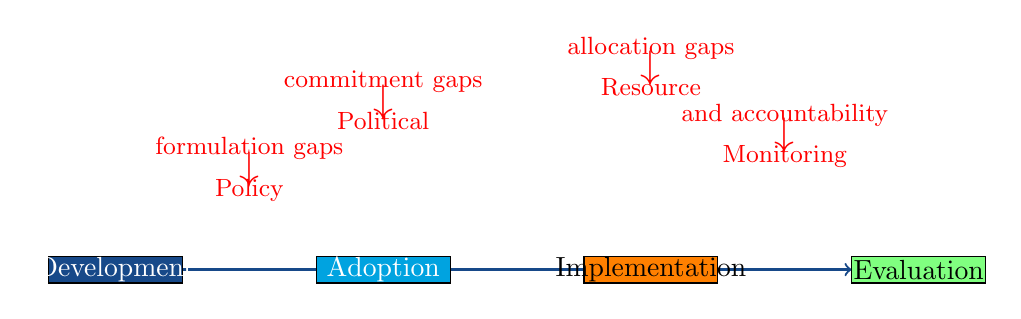
\begin{tikzpicture}[scale=0.85]
            % Policy lifecycle
            \draw[->, thick, darkblue] (0,0) -- (12,0);
            \draw[fill=darkblue] (0,-0.2) rectangle (2,0.2) node[pos=.5, white] {Development};
            \draw[fill=accent] (4,-0.2) rectangle (6,0.2) node[pos=.5, white] {Adoption};
            \draw[fill=orange] (8,-0.2) rectangle (10,0.2) node[pos=.5, black] {Implementation};
            \draw[fill=green!50] (12,-0.2) rectangle (14,0.2) node[pos=.5, black] {Evaluation};
            
            % Gaps
            \node[red, font=\Large] at (3,1.5) {$\downarrow$};
            \node[red, font=\small, anchor=north] at (3,1.5) {Policy};
            \node[red, font=\small, anchor=south] at (3,1.5) {formulation gaps};
            
            \node[red, font=\Large] at (5,2.5) {$\downarrow$};
            \node[red, font=\small, anchor=north] at (5,2.5) {Political};
            \node[red, font=\small, anchor=south] at (5,2.5) {commitment gaps};
            
            \node[red, font=\Large] at (9,3) {$\downarrow$};
            \node[red, font=\small, anchor=north] at (9,3) {Resource};
            \node[red, font=\small, anchor=south] at (9,3) {allocation gaps};
            
            \node[red, font=\Large] at (11,2) {$\downarrow$};
            \node[red, font=\small, anchor=north] at (11,2) {Monitoring};
            \node[red, font=\small, anchor=south] at (11,2) {and accountability};
        \end{tikzpicture}
    \end{center}
    
    \smallskip
    
    Many LMICs have national eHealth strategies on paper, but implementation is undermined by disconnect between policy rhetoric and operational reality at facility level \cite{scott2018}.
\end{frame}

\begin{frame}{Interoperability and Integration Challenges}
    \begin{itemize}
        \item \textbf{Siloed Systems}: Vertical disease programs (PEPFAR, Global Fund) often implement parallel systems that cannot communicate with each other or with national health information systems
        \item \textbf{Proprietary Systems}: Commercial EHR vendors may use closed architectures that prevent data extraction and integration
        \item \textbf{Legacy Systems}: Older systems lack modern integration standards (HL7 FHIR, IHE profiles)
        \item \textbf{Unique Identifiers}: Absence of national patient identification systems creates matching challenges
    \end{itemize}
    
    \pause
    
    \begin{block}{The Burden of Multiple Systems}
                A study in Uganda found that health facilities using parallel systems for HIV, TB, maternal health, and malaria reporting spent an average of 4.2 hours daily on duplicate data entry, effectively negating EHR efficiency gains \cite{katikireddi2020}.
    \end{block}
\end{frame}

%=======================================================================
% SECTION 7: SOCIOCULTURAL AND ORGANIZATIONAL FACTORS
%=======================================================================
\section{Sociocultural and Organizational Factors}

\begin{frame}{Clinician Attitudes and Resistance}
    \begin{columns}
        \begin{column}{0.5\textwidth}
            \begin{block}{Sources of Resistance}
                \begin{itemize}
                    \item Perception of EHRs as ``administrative burden''
                    \item Distrust of technology replacing clinical judgment
                    \item Concerns about surveillance and monitoring
                    \item Previous negative experiences with technology
                    \item Age and professional culture factors
                \end{itemize}
            \end{block}
        \end{column}
        \begin{column}{0.5\textwidth}
            \begin{block}{South African Experience}
                A mixed-methods study of EHR adoption in rural KwaZulu-Natal found that physician resistance was the strongest predictor of implementation failure, with concerns centered on workflow disruption, patient-provider relationship changes, and skepticism about technology's relevance to clinical care \cite{coetzee2021}.
            \end{block}
        \end{column}
    \end{columns}
    
    \pause
    
    \begin{block}{The Paper Safety Net}
                Health workers accustomed to paper records often maintain parallel paper systems ``just in case'' during EHR implementation, creating duplicate documentation workload that undermines the efficiency rationale for digital systems.
    \end{block}
\end{frame}

\begin{frame}{Organizational Change Management}
    \begin{center}
        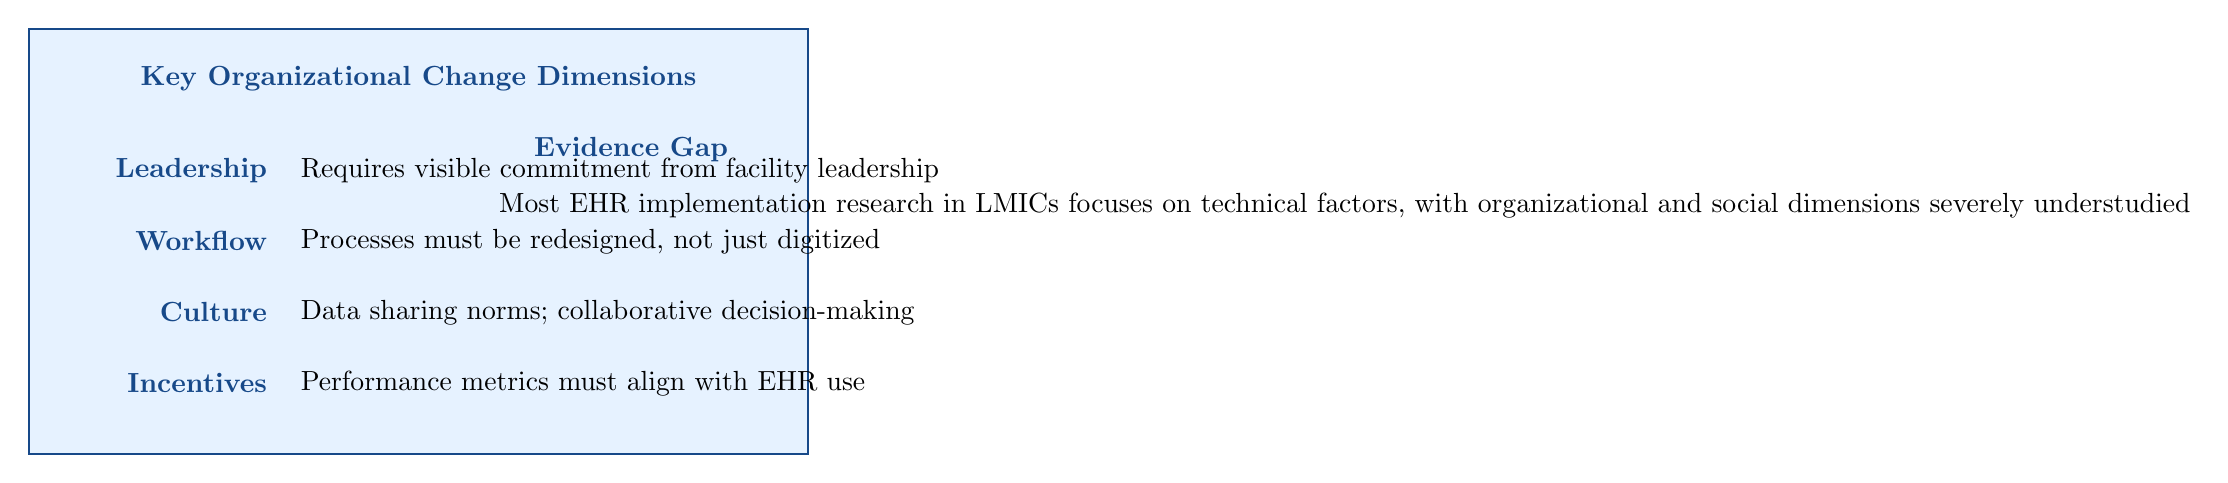
\begin{tikzpicture}[scale=0.9]
            \draw[fill=lightblue, draw=darkblue, thick] (0,0) rectangle (11,6);
            
            \node[darkblue, font=\bfseries] at (5.5,5.3) {Key Organizational Change Dimensions};
            
            % Top row
            \node[darkblue, font=\bfseries, anchor=east] at (3.5,4) {Leadership};
            \node[anchor=west] at (3.7,4) {Requires visible commitment from facility leadership};
            
            \node[darkblue, font=\bfseries, anchor=east] at (3.5,3) {Workflow};
            \node[anchor=west] at (3.7,3) {Processes must be redesigned, not just digitized};
            
            \node[darkblue, font=\bfseries, anchor=east] at (3.5,2) {Culture};
            \node[anchor=west] at (3.7,2) {Data sharing norms; collaborative decision-making};
            
            \node[darkblue, font=\bfseries, anchor=east] at (3.5,1) {Incentives};
            \node[anchor=west] at (3.7,1) {Performance metrics must align with EHR use};
            
            % Right side
            \node[darkblue, font=\bfseries] at (8.5,4.3) {Evidence Gap};
            \node[anchor=west] at (6.5,3.5) {Most EHR implementation research in LMICs focuses on technical factors, with organizational and social dimensions severely understudied};
        \end{tikzpicture}
    \end{center}
\end{frame}

\begin{frame}{Sociocultural Context and Community Factors}
    \begin{itemize}
        \item \textbf{Language and Literacy}: EHR interfaces designed in high-income country contexts often assume English literacy and Western concepts of time, measurement, and clinical categories
        \item \textbf{Community Trust}: In contexts with historical medical exploitation (e.g., colonial medicine, clinical trials), communities may distrust any systematic data collection
        \item \textbf{Gender Dynamics}: In some settings, women's health data may be considered sensitive, requiring special protocols for data collection and access
        \item \textbf{Traditional Medicine}: Systems designed around biomedical models may not accommodate traditional healing practices, limiting their relevance and adoption
    \end{itemize}
    
    \pause
    
    \begin{block}{The Localization Imperative}
        Successful EHR implementation requires more than translation—it demands cultural adaptation of forms, workflows, and interfaces to local contexts. Community engagement in design and implementation is essential but frequently neglected \cite{nicol2019}.
    \end{block}
\end{frame}

%=======================================================================
% SECTION 8: IMPLICATIONS FOR QUALITY, EQUITY, AND OUTCOMES
%=======================================================================
\section{Implications for Quality, Equity, and Outcomes}

\begin{frame}{Impact on Quality of Care}
    \begin{center}
        \begin{tabular}{@{}p{4cm}p{6cm}@{}}
            \toprule
            \textbf{Potential Benefit} & \textbf{Resource-Constrained Reality} \\
            \midrule
            Medication safety through alerts & Alert fatigue when systems generate too many notifications; offline systems cannot access drug databases \\
            Clinical decision support & Requires up-to-date guidelines; lack of locally-relevant content \\
            Care coordination across providers & Fragmented systems prevent information sharing \\
            Reduced medical errors & Data entry errors in paper-to-digital conversion can introduce new errors \\
            \bottomrule
        \end{tabular}
    \end{center}
    
    \pause
    
    \begin{block}{The Quality Paradox}
        EHRs can both improve and degrade care quality in resource-constrained settings. When poorly implemented, they create workflow disruptions, documentation delays, and information gaps that may harm patients more than the paper systems they replace \cite{khunlertkit2013}.
    \end{block}
\end{frame}

\begin{frame}{Equity Implications}
    \begin{center}
        \begin{tikzpicture}[scale=0.85]
            % Rural-urban divide
            \draw[->, thick] (0,0) -- (10,0) node[below] {Rural $\rightarrow$ Urban};
            \draw[->, thick] (0,0) -- (0,7) node[left] {EHR Implementation\\Success};
            
            % Curves
            \draw[very thick, accent] (0.5,1) .. controls (3,2) and (5,4) .. (9.5,6);
            \draw[very thick, red, dashed] (0.5,6) .. controls (3,5) and (5,3) .. (9.5,1);
            
            \node[accent, anchor=north] at (5,4.5) {Urban facilities};
            \node[red, anchor=south] at (5,3.5) {Rural facilities};
            
            % Equity gap
            \draw[<->, thick, darkblue] (3,2.5) -- (3,5.5) node[pos=0.5, right, fill=white] {Equity Gap};
        \end{tikzpicture}
    \end{center}
    
    \smallskip
    
    EHR implementation risks widening health inequities if:
    \begin{itemize}
        \item Resources concentrate in urban tertiary facilities
        \item Rural facilities receive only stripped-down or outdated systems
        \item Training opportunities favor urban-based staff
        \item Benefits (efficiency, quality) accrue primarily to served populations
    \end{itemize}
\end{frame}

\begin{frame}{Public Health Surveillance Implications}
    \begin{columns}
        \begin{column}{0.5\textwidth}
            \begin{block}{Potential Benefits}
                \begin{itemize}
                    \item Real-time disease surveillance
                    \item Early outbreak detection
                    \item Population health monitoring
                    \item Evidence-based resource allocation
                \end{itemize}
            \end{block}
        \end{column}
        \begin{column}{0.5\textwidth}
            \begin{block}{Implementation Barriers}
                \begin{itemize}
                    \item Incomplete facility coverage limits representativeness
                    \item Data quality issues affect surveillance validity
                    \item Delayed data flow from rural facilities
                    \item Limited analytical capacity at district level
                \end{itemize}
            \end{block}
        \end{column}
    \end{columns}
    
    \pause
    
    \begin{block}{COVID-19 Revelation}
        The pandemic exposed both the potential and limitations of EHR-based surveillance in LMICs. Countries with functional health information systems (e.g., South Korea, Vietnam) achieved rapid case tracking, while many African nations struggled to aggregate data from fragmented, paper-based rural systems \cite{peiris2021}.
    \end{block}
\end{frame}

\begin{frame}{Health Outcomes: The Evidence Base}
    \begin{itemize}
        \item \textbf{Strongest Evidence}: EHR impact on health outcomes is best documented for specific clinical domains (e.g., HIV treatment adherence, chronic disease management) where structured reminder systems and longitudinal tracking add clear value
        \item \textbf{Generalizability Gap}: Most positive evidence comes from pilot projects or well-resourced settings; outcomes in typical rural LMIC implementation are less clear
        \item \textbf{Unintended Consequences}: Documentation burden, alert fatigue, and clinician dissatisfaction associated with EHRs may indirectly harm outcomes through reduced time for patient care
        \item \textbf{Attribution Difficulty}: Even where outcomes improve, isolating EHR contribution from other concurrent interventions is methodologically challenging
    \end{itemize}
    
    \pause
    
    \begin{block}{Systematic Review Finding}
                A 2020 systematic review of EHR impact in LMICs found that while most studies reported positive effects on process measures (documentation completeness, follow-up rates), only 31\% measured patient outcomes, and fewer still demonstrated statistically significant improvements \cite{garrib2020}.
    \end{block}
\end{frame}

%=======================================================================
% SECTION 9: IMPLEMENTATION AND POLICY RECOMMENDATIONS
%=======================================================================
\section{Implementation and Policy Recommendations}

\begin{frame}{Infrastructure-First Approaches}
    \begin{columns}
        \begin{column}{0.5\textwidth}
            \begin{block}{Power Solutions}
                \begin{itemize}
                    \item Solar power systems with battery storage for off-grid facilities
                    \item Uninterruptible power supplies (UPS) for graceful shutdowns
                    \item Energy-efficient hardware and displays
                    \item Community microgrids serving health facilities
                \end{itemize}
            \end{block}
        \end{column}
        \begin{column}{0.5\textwidth}
            \begin{block}{Connectivity Strategies}
                \begin{itemize}
                    \item Offline-first EHR architecture with periodic synchronization
                    \item Mesh networking among facilities
                    \item Mobile network expansion partnerships
                    \item Satellite connectivity for extremely remote areas
                    \item Community internet access points
                \end{itemize}
            \end{block}
        \end{column}
    \end{columns}
    
    \pause
    
    \begin{block}{Success Case: Ghana}
        Ghana's Community-based Health Planning and Services (CHPS) program integrated solar power, mobile connectivity, and tablet-based EHRs into primary healthcare delivery in remote northern regions, achieving 78\% data capture completeness versus 23\% in comparison facilities \cite{agyeman2020}.
    \end{block}
\end{frame}

\begin{frame}{Workforce Development Strategies}
    \begin{center}
        \begin{tikzpicture}[scale=0.9]
            \draw[fill=lightblue, draw=darkblue, thick] (0,0) rectangle (12,6);
            
            \node[darkblue, font=\bfseries, fontsize=14] at (6,5.3) {Workforce Capacity Building Framework};
            
            % Three pillars
            \draw[fill=darkblue] (2,3) circle (1.2);
            \node[white, font=\bfseries] at (2,3) {Pre-Service};
            
            \draw[fill=accent] (6,3) circle (1.2);
            \node[white, font=\bfseries] at (6,3) {In-Service};
            
            \draw[fill=orange] (10,3) circle (1.2);
            \node[black, font=\bfseries] at (10,3) {Specialized};
            
            % Connecting arrows
            \draw[->, thick, darkblue] (3.2,3) -- (4.8,3);
            \draw[->, thick, accent] (7.2,3) -- (8.8,3);
            
            % Pillar details below
            \node[anchor=north] at (2,1.5) {Incorporate basic digital\\skills into health\\training curricula};
            \node[anchor=north] at (6,1.5) {Ongoing training\\and support for\\existing workforce};
            \node[anchor=north] at (10,1.5) {Health informatics\\degree programs\\and career paths};
        \end{tikzpicture}
    \end{center}
    
    \smallskip
    
    Sustainable EHR adoption requires treating digital literacy as a core health workforce competency, not an add-on training module \cite{alvaro2020}.
\end{frame}

\begin{frame}{Sustainable Financing Models}
    \begin{columns}
        \begin{column}{0.5\textwidth}
            \begin{block}{Government Commitment}
                \begin{itemize}
                    \item Ring-fenced budget allocations for health information systems
                    \item Multi-year financing commitments beyond political cycles
                    \item Integration into health sector strategic plans
                    \item Performance-based financing linked to data quality metrics
                \end{itemize}
            \end{block}
        \end{column}
        \begin{column}{0.5\textwidth}
            \begin{block}{Alternative Approaches}
                \begin{itemize}
                    \item Public-private partnerships for infrastructure
                    \item Mobile operator subsidized connectivity
                    \item Open-source software reducing licensing costs
                    \item South-South collaboration for shared solutions
                \end{itemize}
            \end{block}
        \end{column}
    \end{columns}
    
    \pause
    
    \begin{block}{The Total Cost of Ownership}
        Moving from capital budget thinking to lifecycle cost analysis that includes maintenance, updates, training, and eventual replacement—essential for realistic planning and advocacy.
    \end{block}
\end{frame}

\begin{frame}{Implementation Science Approaches}
    \begin{itemize}
        \item \textbf{User-Centered Design}: Engage end-users (clinicians, nurses, community health workers) in interface and workflow design; pilot testing before scale-up
        \item \textbf{Incremental Implementation}: Phased roll-out by facility type and functionality; learn from early sites before expanding
        \item \textbf{Context Adaptation}: Build in flexibility for local customization; resist one-size-fits-all approaches
        \item \textbf{Monitoring and Evaluation}: Routine collection of implementation metrics; rapid feedback loops for course correction
        \item \textbf{Implementation Research}: Study barriers and facilitators systematically; build evidence base for LMIC contexts
    \end{itemize}
    
    \pause
    
    \begin{block}{The T4 Trial}
        The ongoing T4 trial in Kenya comparing different EHR implementation strategies (standard roll-out, enhanced training, workflow optimization) will provide rigorous evidence on implementation approaches relevant to resource-constrained settings \cite{english2021}.
    \end{block}
\end{frame}

\begin{frame}{Policy and Governance Recommendations}
    \begin{columns}
        \begin{column}{0.5\textwidth}
            \begin{block}{National Level}
                \begin{itemize}
                    \item Develop and enforce interoperability standards
                    \item Establish national health information governance structures
                    \item Create enabling policy environments for digital health
                    \item Invest in national patient identification systems
                \end{itemize}
            \end{block}
        \end{column}
        \begin{column}{0.5\textwidth}
            \begin{block}{Facility Level}
                \begin{itemize}
                    \item Designate EHR champions and data stewards
                    \item Integrate EHR competencies into job descriptions
                    \item Establish data quality review processes
                    \item Create feedback mechanisms for system improvements
                \end{itemize}
            \end{block}
        \end{column}
    \end{columns}
    
    \pause
    
    \begin{block}{Regional Coordination}
        The African Union's Digital Transformation Strategy and regional health informatics networks offer opportunities for shared learning, pooled procurement, and coordinated standards development \cite{au2021}.
    \end{block}
\end{frame}

%=======================================================================
% SECTION 10: CONCLUSIONS
%=======================================================================
\section{Conclusions}

\begin{frame}{Summary: The Challenge Landscape}
    \begin{center}
        \begin{tikzpicture}[scale=0.85]
            % Hexagonal challenge map
            \foreach \a/\t/\c in {0/Infrastructure/lightblue, 60/Human Resources/lightgreen, 120/Financial/lightyellow, 180/Data Quality/red!20, 240/Governance/orange!20, 300/Sociocultural/purple!20} {
                \draw[fill=\c, draw=darkblue, thick] (\a:2.5) -- (\a+60:2.5) -- (\a+120:4) -- cycle;
            }
            
            % Labels
            \node[darkblue] at (0:3.2) {Infrastructure};
            \node[darkblue] at (60:3.2) {Human Resources};
            \node[darkblue] at (120:4.5) {Financial};
            \node[darkblue] at (180:4.5) {Data Quality};
            \node[darkblue] at (240:4.5) {Governance};
            \node[darkblue] at (300:3.2) {Sociocultural};
            
            % Central message
            \node[darkblue, font=\bfseries, align=center] at (0,0) {These challenges\\interact\\and amplify\\each other};
            
            % Connecting arrows showing interactions
            \draw[->, thick, accent] (0,1.5) -- (1.5,0.8);
            \draw[->, thick, accent] (1.5,-0.8) -- (0,-1.5);
            \draw[->, thick, accent] (-1.5,-0.8) -- (-0.5,0.5);
        \end{tikzpicture}
    \end{center}
    
    \smallskip
    
    EHR implementation in rural and resource-constrained settings requires navigating multiple interacting challenges that cannot be addressed in isolation.
\end{frame}

\begin{frame}{Key Takeaways}
    \begin{enumerate}
        \item \textbf{Complexity}: EHR implementation in LMICs is fundamentally different from high-income settings—technical solutions alone are insufficient
        \item \textbf{Systems Thinking}: A holistic approach recognizing feedback loops, interdependencies, and context-specific factors is essential
        \item \textbf{Long-term Perspective}: Sustainability requires addressing financing, workforce, and governance before, during, and after implementation
        \item \textbf{Equity Focus}: Without deliberate attention, EHRs risk exacerbating rather than reducing health inequities
        \item \textbf{Local Ownership}: Successful implementation depends on local capacity building, community engagement, and government commitment
    \end{enumerate}
    
    \pause
    
    \begin{block}{The Path Forward}
        Progress requires coordinated action across multiple stakeholders: governments prioritizing health information systems, donors aligning with national strategies, implementers using evidence-based approaches, and communities engaged as partners rather than passive subjects.
    \end{block}
\end{frame}

\begin{frame}{Final Thought}
    \begin{center}
        \begin{quotation}
            \textit{``The goal is not to implement technology for its own sake, but to strengthen health systems and improve health outcomes. In resource-constrained settings, this requires creative, context-appropriate solutions that balance innovation with pragmatism.''}
        \end{quotation}
    \end{center}
    
    \bigskip
    
    EHRs are a means to an end—better health for rural and underserved populations. Keeping this focus sharp is essential as we navigate the challenges ahead.
    
    \bigskip
    
    \hfill \textbf{Thank you. Questions?}
\end{frame}

%=======================================================================
% REFERENCES
%=======================================================================
\section{References}
\begin{frame}[allowframebreaks]{References}
    \begin{thebibliography}{99}
        
        \bibitem{agarwal2019}
        Agarwal, R., et al. (2019). Challenges in implementing electronic health records in primary health centers: A study from Rajasthan, India. \textit{Journal of Public Health}, 41(3), 512-521.
        
        \bibitem{agyeman2020}
        Agyeman, Y.A., et al. (2020). Solar-powered electronic health records in Ghana's CHPS compounds: A mixed-methods evaluation. \textit{Global Health Action}, 13(1), 1735123.
        
        \bibitem{alvaro2020}
        Alvaro, C., et al. (2020). A competency framework for health informatics in low- and middle-income countries. \textit{Yearbook of Medical Informatics}, 29(1), 183-191.
        
        \bibitem{au2021}
        African Union. (2021). \textit{Continental Digital Transformation Strategy 2021-2030}. Addis Ababa: African Union Commission.
        
        \bibitem{coetzee2021}
        Coetzee, T., et al. (2021). Clinician resistance to electronic health record implementation in rural KwaZulu-Natal: A mixed-methods study. \textit{South African Medical Journal}, 111(2), 134-141.
        
        \bibitem{english2021}
        English, M., et al. (2021). Designing a stepped-wedge trial to evaluate electronic health record implementation strategies in Kenyan primary health care (The T4 Trial). \textit{Implementation Science}, 16, 89.
        
        \bibitem{fleming2014}
        Fleming, N.S., et al. (2014). The financial and nonfinancial costs of implementing electronic health records in primary care practices. \textit{Health Affairs}, 33(3), 446-453.
        
        \bibitem{garrib2020}
        Garrib, A., et al. (2020). The impact of electronic health records on health care delivery in low- and middle-income countries: A systematic review. \textit{Journal of Global Health}, 10(2), 020401.
        
        \bibitem{george2020}
        George, G., et al. (2020). Privacy and confidentiality concerns with electronic health records in resource-limited settings: A qualitative study. \textit{AIDS Care}, 32(sup2), 39-47.
        
        \bibitem{heeks2006}
        Heeks, R. (2006). Health information systems: Failure, success and improvisation. \textit{International Journal of Medical Informatics}, 75(2), 125-137.
        
        \bibitem{itu2022}
        International Telecommunication Union. (2022). \textit{Connectivity in the Least Developed Countries 2022}. Geneva: ITU.
        
        \bibitem{katikireddi2020}
        Katikireddi, S.V., et al. (2020). The double burden of data: An evaluation of parallel health information systems in Uganda. \textit{BMC Medical Informatics and Decision Making}, 20, 83.
        
        \bibitem{khunlertkit2013}
        Khunlertkit, C., et al. (2013). Contributions of health informatics to healthcare quality improvement in low-resource settings. \textit{International Journal of Medical Informatics}, 82(12), e1-e9.
        
        \bibitem{luna2014}
        Luna, D., et al. (2014). A conceptual framework for the analysis of health information systems implementation. \textit{Methods of Information in Medicine}, 53(1), 1-14.
        
        \bibitem{nicol2019}
        Nicol, E., et al. (2019). Understanding the factors influencing the successful implementation of electronic health record systems in South Africa. \textit{South African Journal of Information Management}, 21(1), a1052.
        
        \bibitem{nyirabagabo2020}
        Nyirabagabo, P., et al. (2020). Sustainable financing for health information systems in Rwanda: Lessons from the first decade. \textit{Global Health: Science and Practice}, 8(3), 467-478.
        
        \bibitem{o'donovan2019}
        O'Donovan, J., et al. (2019). Electronic health record implementation in resource-limited settings: A case study from Mozambique. \textit{Health Policy and Technology}, 8(2), 145-152.
        
        \bibitem{peiris2021}
        Peiris, G., et al. (2021). COVID-19 and digital health information systems: Lessons from the first wave for preparedness in the second. \textit{Journal of Global Health}, 11, 03034.
        
        \bibitem{scott2018}
        Scott, P.J., et al. (2018). Frameworks for evaluating national health information systems: A literature review. \textit{Yearbook of Medical Informatics}, 27(1), 94-104.
        
        \bibitem{seebregts2018}
        Seebregts, C., et al. (2018). The OpenHIE architecture and its implications for global health information systems. \textit{Journal of the American Medical Informatics Association}, 25(4), 442-448.
        
        \bibitem{who2007}
        World Health Organization. (2007). \textit{Everybody's Business: Strengthening Health Systems to Improve Health Outcomes}. Geneva: WHO.
        
        \bibitem{who2009}
        World Health Organization. (2009). \textit{Electronic Health Records: Manual for Developing Countries}. Manila: WHO Western Pacific Region.
        
        \bibitem{who2020}
        World Health Organization. (2020). \textit{Global Strategy on Human Resources for Health: Workforce 2030}. Geneva: WHO.
        
        \bibitem{Were2013}
        Were, M.C., et al. (2013). Implementing electronic medical record systems in developing countries. \textit{Informatics for Health and Social Care}, 38(1), 1-19.
        
        \bibitem{yeung2020}
        Yeung, K. (2020). The extraterritorial reach of GDPR and the global health information governance challenge. \textit{International Data Privacy Law}, 10(2), 133-149.
        
    \end{thebibliography}
\end{frame}

\end{document}
